\definecolor{srblue}{RGB}{196,124,73}
\definecolor{srgreenfill}{RGB}{255,244,232}
\definecolor{srgreendraw}{RGB}{198,132,76}
\definecolor{srorangefill}{RGB}{255,236,214}
\definecolor{srorangedraw}{RGB}{221,132,59}
\definecolor{srgrayfill}{RGB}{252,245,238}
\definecolor{srgraydraw}{RGB}{141,118,100}
\definecolor{srhwfill}{RGB}{245,233,221}
\definecolor{srtext}{RGB}{34,38,45}

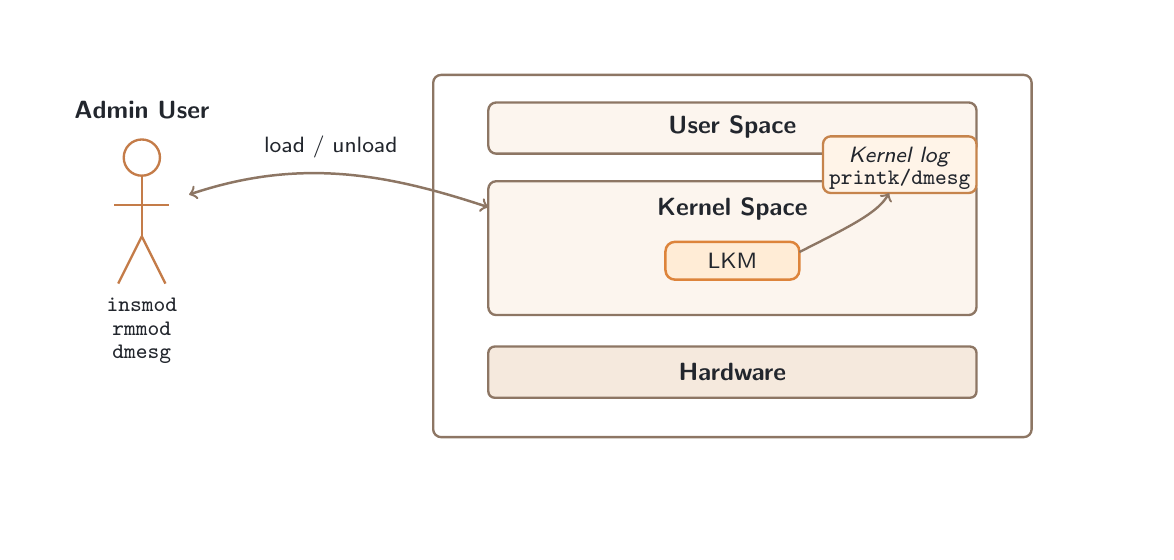
\begin{tikzpicture}[
  x=1cm,
  y=1cm,
  every node/.style={inner sep=0pt, outer sep=0pt},
  label/.style={font=\sffamily\fontsize{8}{8.6}\selectfont, text=srtext, align=center},
  title/.style={font=\sffamily\bfseries\fontsize{9}{9.6}\selectfont, text=srtext, align=center},
  block/.style={draw=srgraydraw, rounded corners=0.10cm, line width=0.85pt},
  kernelbox/.style={draw=srorangedraw, fill=srorangefill, rounded corners=0.12cm, line width=0.9pt},
  softbox/.style={draw=srgraydraw, fill=srgrayfill, rounded corners=0.10cm, line width=0.85pt},
  hwbox/.style={draw=srgraydraw, fill=srhwfill, rounded corners=0.08cm, line width=0.85pt},
  logbox/.style={draw=srgreendraw, fill=srgreenfill, rounded corners=0.10cm, line width=0.85pt},
  flow/.style={draw=srgraydraw, line width=0.9pt, <->}
]

  \path[use as bounding box] (0,0) rectangle (14.2,6.4);

  % Admin user
  \draw[srblue, line width=0.85pt] (1.45,4.75) circle (0.23);
  \draw[srblue, line width=0.85pt] (1.45,4.50) -- (1.45,3.75);
  \draw[srblue, line width=0.85pt] (1.10,4.15) -- (1.80,4.15);
  \draw[srblue, line width=0.85pt] (1.45,3.75) -- (1.15,3.15);
  \draw[srblue, line width=0.85pt] (1.45,3.75) -- (1.75,3.15);
  \node[title] at (1.45,5.35) {Admin User};
  \node[label] at (1.45,2.55) {\texttt{insmod}\\\texttt{rmmod}\\\texttt{dmesg}};

  % Main system block
  \draw[block] (5.15,1.20) rectangle (12.75,5.80);

  \draw[softbox] (5.85,4.80) rectangle (12.05,5.45);
  \node[title] at (8.95,5.13) {User Space};

  \draw[softbox] (5.85,2.75) rectangle (12.05,4.45);
  \node[title] at (8.95,4.10) {Kernel Space};
  \draw[kernelbox] (8.10,3.20) rectangle (9.80,3.68);
  \node[label] at (8.95,3.44) {LKM};

  \draw[logbox] (10.10,4.30) rectangle (12.05,5.02);
  \node[label] at (11.075,4.76) {\textit{Kernel log}};
  \node[label] at (11.075,4.48) {\texttt{printk/dmesg}};
  \draw[draw=srgraydraw, line width=0.85pt, ->]
    (9.80,3.55) .. controls (10.45,3.88) and (10.80,4.05) .. (10.94,4.30);

  \draw[hwbox] (5.85,1.70) rectangle (12.05,2.35);
  \node[title] at (8.95,2.03) {Hardware};

  % Arrows
  \draw[flow] (2.05,4.28) .. controls (3.45,4.75) and (4.55,4.55) .. (5.85,4.12);
  \node[label] at (3.85,4.88) {load / unload};

\end{tikzpicture}
